\scanpage{15}\mspage{14}
% ink top, relations
If one is given the two relations at the same time
\[
\left\{\begin{aligned}
\unsure{\underline R|R}(a,b)&\qquad \{a,b\}\in\mathrm{Drap}_2(\mathcal L)\\
R(a,b,c)&\qquad b\text{ is strictly between }a\text{ and }c
\end{aligned}\right.
\]
then to recover the biorder, it suffices to assume $\mathcal L$ upward filtering and downward filtering, \deleted{and the relations \unsure{If|if}, \unsure{This|this|Oct} \unsure{on the}, \unsure{upward} and \unsure{downward} filtering \unsure{are} of \unsure{some|all} \unsure{components|ways} \unsure{connected|known in} \unsure{$S_0$|$v_0$|$0$}} 

% ink middle, On va voir
\deleted{\unsure{We are going to}} We are going to see now how knowledge\inserted{ of $\mathrm{Drap}_2(\mathcal L)$, and} for $\unsure{\varepsilon|\mathcal E|E}\in\mathrm{Drap}_2(\deleted{\unsure{I}}\mathcal L)$, of the decomposition of
% ink middle, C(\unsure{\varepsilon|\mathcal E|E}) and continuation
\[
 C(\unsure{\varepsilon|\mathcal E|E})=\{\,t\in\mathcal L\deleted{\unsure{\notin\varepsilon|\smallsetminus\varepsilon}}\mid
 \deleted{\unsure{x}}\{\unsure{\varepsilon|\mathcal E|E}\unsure{\cup|,}t\}\deleted{\unsure{=|-}}\in\mathrm{Drap}_3(\mathcal L)\,\}
\]
into connected components, implies knowledge of the relation
\[
 R(a,b,c)\unsure{\mathord{:}|\mathord{?}}\quad b\text{ strictly between }a\text{ and }c.
\]
% ink lower third, Première condition
First condition : $\{a,b,c\}\in\mathrm{Drap}_3(\mathcal L)$ (follows from the datum of $\mathrm{Drap}_2(\mathcal L)$)
\figure{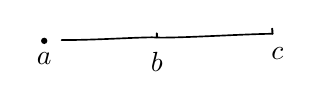
\begin{tikzpicture}[x=1cm,y=1cm,line cap=round]
\fill (0,0) circle (1.15pt);
\draw[line width=.6pt] (.22,.01) .. controls (.66,.01) and (1.06,.04) .. (1.37,.045) .. controls (1.61,.026) and (2.48,.085) .. (2.9,.09);
\draw[line width=.7pt] (1.43,.045) -- (1.43,.095) (2.9,.09) -- (2.895,.155);
\node[below] at (0,-.025) {$a$};
\node[below] at (1.43,-.015) {$b$};
\node[below] at (2.96,.035) {$c$};
\end{tikzpicture}}
% ink bottom, final sentence and cancelled display
If $b$ is between $a$ and $c$, let us look at the
\[
 \deleted{J_{abc}=\text{component of }C(\{a,b\}}\unsure{,|)}
\]

% pale vertical watermark
% the paper's watermark (EXTRA STRONG), not his text
